\documentclass[a4paper,12pt]{article}

\usepackage[utf8]{inputenc}
\usepackage[T1]{fontenc}
\usepackage[french]{babel}
\usepackage{graphicx}
\usepackage{hyperref}
\usepackage{geometry}
\usepackage{csquotes}
\usepackage{hhline}
\usepackage{biblatex}
\usepackage{caption}
\usepackage{subcaption}
\usepackage{float}
\addbibresource{project.bib}
\geometry{margin=2.5cm}
\DeclareUnicodeCharacter{0302}{\^{} }

\usepackage{tikz}
\usetikzlibrary{shapes.geometric, arrows, positioning}

\title{
    
\includegraphics[width=4cm]{logo.jpg}\\[1cm]
    Rapport TP Programmation Orientée Objet : \\
    \textbf{Projet MeetingPro}
}
\author{
    GRIMM-KEMPF Matthieu \\
    DAGON Lucas
}
\date{\today}

\begin{document}

\maketitle

\begin{abstract}
    Ce rapport présente le développement du projet MeetingPro, réalisé dans le cadre du cours de Programmation Orientée Objet. Nous y détaillons la démarche de conception, les choix techniques, la répartition des tâches, les difficultés rencontrées ainsi que les résultats obtenus.
\end{abstract}

\tableofcontents
\newpage

\section{Introduction}
Ce projet vise à développer une application de gestion de salles de réunion en utilisant les principes de la programmation orientée objet. L'objectif est de fournir une solution robuste et évolutive pour la gestion des réservations de salles.

\section{Méthodologie}

Le développement de l'application s’est appuyé sur une approche structurée inspirée du modèle MVC (Modèle-Vue-Contrôleur). Notre priorité a été d’assurer une séparation claire entre les différents composants pour favoriser maintenabilité, évolutivité et testabilité du code.

\subsection{Répartition du travail}

La répartition du travail a été définie dès les premières étapes du projet :
\begin{itemize}
    \item \textbf{GRIMM-KEMPF Matthieu} s’est chargé de la partie \textit{Contrôleur}, du \textit{Modèle}, du script d’installation du package, des scripts de tests, ainsi que de l’intégralité de la documentation (README et rapport).
    \item \textbf{DAGON Lucas} a développé l'\textit{interface graphique} en utilisant la bibliothèque Tkinter.
\end{itemize}

\subsection{Communication et gestion de version}

La coordination entre les membres s’est effectuée principalement via \textbf{Discord}, avec des points réguliers pour suivre l’avancée des travaux. Pour la gestion de version, nous avons utilisé \textbf{Git} avec un dépôt hébergé sur \textbf{GitHub}, conformément aux recommandations de nos enseignants.

\subsection{Choix techniques et architecture}

L'application est écrite en Python et utilise :
\begin{itemize}
    \item \textbf{Tkinter} pour l’interface graphique, qui, bien que rudimentaire, offre suffisamment de fonctionnalités
          pour réaliser une interface fonctionnelle.\item \textbf{Hmac} pour la génération d'ID pour l'utilisateur. La génération d'ID ne passe pas par UUID mais par SHA256 pour réutiliser du code déjà écris pour un projet personnel. Cette méthode ne garanti certe pas un ID unique malgré qu'une chance inférieure à $1.0\cdot 10^{-6}\%$ mais le code l'entourant protège contre ce risque.
    \item \textbf{JSON} pour la persistance des données,
    \item \textbf{HMAC avec SHA-256} pour la génération d'identifiants utilisateurs. Contrairement à l'utilisation de UUID, nous avons opté pour une méthode basée sur HMAC pour réutiliser du code existant d'un projet personnel. Bien que cette méthode ne garantisse pas une unicité absolue des identifiants, la probabilité de collision est extrêmement faible (inférieure à $1.0 \cdot 10^{-6}\%$). De plus, des mécanismes de protection ont été mis en place pour gérer ce risque résiduel.
    \item une architecture \textbf{MVC} bien structurée.
\end{itemize}

Les entités principales (utilisateurs, salles) sont modélisées sous forme de classes, avec sérialisation personnalisée dans des fichiers JSON séparés pour plus de clarté et modularité.

\subsection{Cycle de développement}

Notre démarche fut itérative, avec les étapes suivantes :
\begin{enumerate}
    \item Spécification des fonctionnalités principales,
    \item Modélisation UML des entités,
    \item Développement incrémental avec tests intégrés,
    \item Intégration des différentes parties,
    \item Rédaction de la documentation.
\end{enumerate}

\section{Fonctionnement du système} \label{fonction_sys}

Le projet repose sur une architecture conforme au modèle MVC. Le diagramme suivant illustre les relations entre les composants :

\begin{figure}[H]
    \centering
    \begin{tikzpicture}
        \tikzstyle{box} = [rectangle, draw, fill=blue!20, text centered, minimum height=1.5cm, minimum width=2.5cm]
        \tikzstyle{arrow} = [thick,->,>=stealth]

        \node (interface) [box] {Interface Graphique};
        \node (controleur) [box, right of=interface, xshift=3.5cm] {Contr\^oleur};
        \node (src) [box, right of=controleur, xshift=3cm] {Mod\`ele};

        \node (interactions) [box, below of=interface, yshift=-1.5cm] {Interactions Utilisateur};
        \node (fonctions) [box, below of=controleur, yshift=-1.5cm] {Fonctions Backend};
        \node (logique) [box, below of=src, yshift=-1.5cm] {Logique Syst\`eme};

        \draw [arrow] (interface) -- (controleur);
        \draw [arrow] (controleur) -- (src);
        \draw [arrow] (interface) -- (interactions);
        \draw [arrow] (controleur) -- (fonctions);
        \draw [arrow] (src) -- (logique);
    \end{tikzpicture}
    \caption{Diagramme des relations entre les composants MVC}
    \label{fig:mvc}
\end{figure}

Pour le Modèle, deux groupes de classes ont été définis.

\newpage
\subsection{Gestion des utilisateurs}

La classe \textbf{Person} gère les informations des clients ainsi que leurs réservations. Elle
permet l’ajout, la suppression et la consultation de réservations, ainsi que la sauvegarde
dans un fichier JSON.

\begin{figure}[H]
    \centering
    \begin{tikzpicture}
        \tikzstyle{class} = [rectangle, draw, text width=8cm, text centered, minimum height=1.5cm, minimum width=2.5cm]
        \node (person) [class] {
            \textbf{Person} \\
            \rule{\linewidth}{0.4pt}
            - firstname: str \\
            - sirname: str \\
            - name: str \\
            - email: str \\
            - reservations: dict \\
            - id: str \\
            - file\_path: str \\
            \rule{\linewidth}{0.4pt}
            + \_\_init\_\_(firstname: str, sirname: str, email: str) \\
            + add\_reservation(reservation\_data: dict) -> None \\
            + remove\_reservation(reservation\_data: dict) -> None \\
            + get\_reservations() -> dict \\
            + id\_generator() -> None \\
            + \_\_str\_\_() -> str \\
            + \_\_repr\_\_() -> str \\
            + save\_to\_file() -> None \\
            + from\_save(json\_data) -> Person \\
            + void\_person() -> Person \\
            + from\_search(ID: str) -> Person \\
        };
    \end{tikzpicture}
    \caption{Diagramme de gestion des utilisateurs}
    \label{fig:users}
\end{figure}
\newpage
\subsection{Gestion des salles}

La classe \textbf{Standard} définit les fonctionnalités communes à toutes les salles.\\
Deux classes héritant de \textbf{Standard} spécialisent son comportement pour l’adapter aux
types de salles également disponibles à la location: \textbf{Conference} vérifie que la salle n’est
pas surdimensionnée pour l’événement, et \textbf{ComputerRoom} liste les équipements informa-
tiques disponibles dans ce type de salle.\\
La représentation de ces classes et de leurs relations est la suivante:

\begin{figure}[H]
    \centering
    \begin{tikzpicture}
        \tikzstyle{class} = [rectangle, draw, text width=7cm, text centered, minimum height=1.5cm, minimum width=2.5cm]

        \node (standard) [class] {
            \textbf{Standard} \\
            \rule{\linewidth}{0.4pt}
            - name: str \\
            - capacity: int \\
            - reservations: dict \\
            - file\_path: str \\
            \rule{\linewidth}{0.4pt}
            + \_\_init\_\_(name: str, capacity: int, reservations: dict) \\
            + \_\_str\_\_() -> str \\
            + \_\_repr\_\_() -> str \\
            + too\_small(number\_of\_people: int) -> bool \\
            + reservation\_duration\_valid(duration: int) -> bool \\
            + return\_type() -> str \\
            + add\_reservation(bloc: dict) -> None \\
            + remove\_reservation(bloc: dict) -> bool \\
            + get\_reservations() -> dict \\
            + save\_to\_file() -> None \\
            + load\_from\_json(room\_name: str) -> Standard \\
        };

        \node (conference) [class, below left=1cm and -3cm of standard] {
            \textbf{Conference} \\
            \rule{\linewidth}{0.4pt}
            \rule{\linewidth}{0.4pt}
            + \_\_init\_\_(name: str, capacity: int) \\
            + \_\_str\_\_() -> str \\
            + \_\_repr\_\_() -> str \\
            + too\_big(number\_of\_people: int) -> bool \\
            + return\_type() -> str \\
        };

        \node (computerroom) [class, below right=1cm and -3cm of standard] {
            \textbf{ComputerRoom} \\
            \rule{\linewidth}{0.4pt}
            - equipment: list \\
            \rule{\linewidth}{0.4pt}
            + \_\_init\_\_(name: str, capacity: int) \\
            + return\_equipment() -> str \\
            + \_\_str\_\_() -> str \\
            + \_\_repr\_\_() -> str \\
            + return\_type() -> str \\
        };

        \draw [->] (conference) -- (standard);
        \draw [->] (computerroom) -- (standard);
    \end{tikzpicture}
    \caption{Diagramme de gestion des salles}
    \label{fig:rooms}
\end{figure}

\section{Résultats obtenus}

L’application MeetingPro permet les fonctionnalités suivantes :
\begin{itemize}
    \item Création, modification et suppression d’utilisateurs,
    \item Ajout et gestion de réservations de salles,
    \item Affichage dynamique des informations (utilisateurs, salles, réservations),
    \item Sauvegarde automatique dans des fichiers JSON distincts,
    \item Interface graphique interactive respectant les exigences fonctionnelles.
\end{itemize}

\vspace{1cm}
\textbf{Aperçu de l’application (extraits d’écran)} :

\begin{figure}[H]
    \centering
    \begin{subfigure}{0.8\textwidth}
        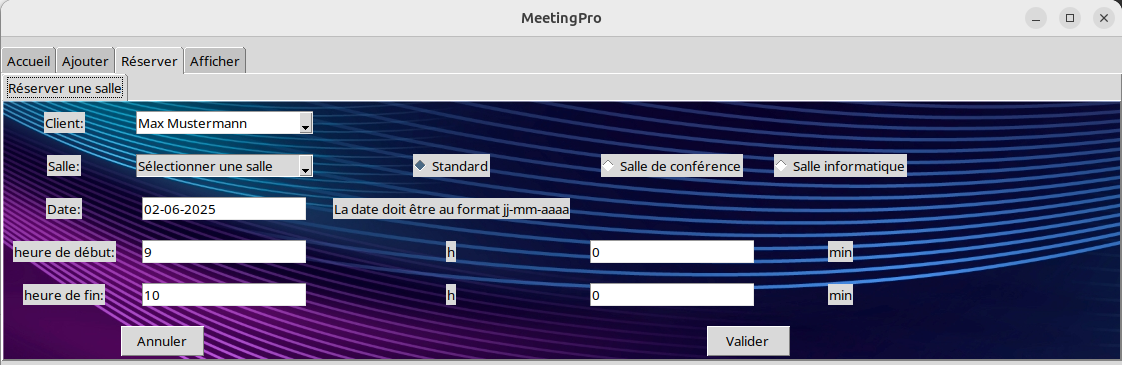
\includegraphics[width=\textwidth]{screenshot1.jpg}
        \caption{Écran de réservation}
    \end{subfigure}
    \hfill
    \begin{subfigure}{0.8\textwidth}
        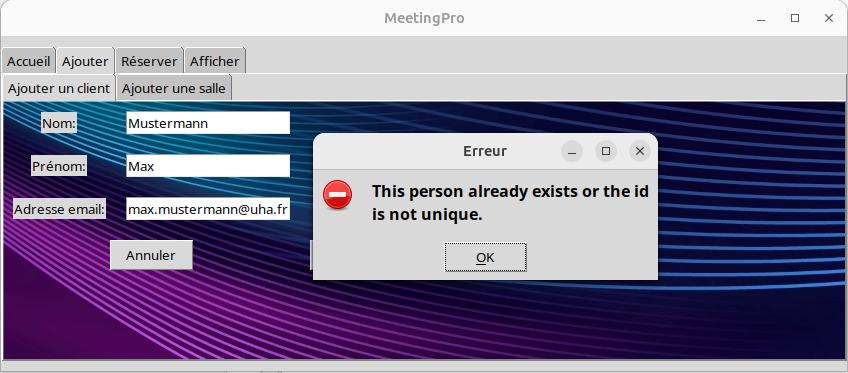
\includegraphics[width=\textwidth]{screenshot2.jpg}
        \caption{Erreur si l'on tente d'ajouter à nouveau un même client}
    \end{subfigure}
    \hfill
    \begin{subfigure}{0.8\textwidth}
        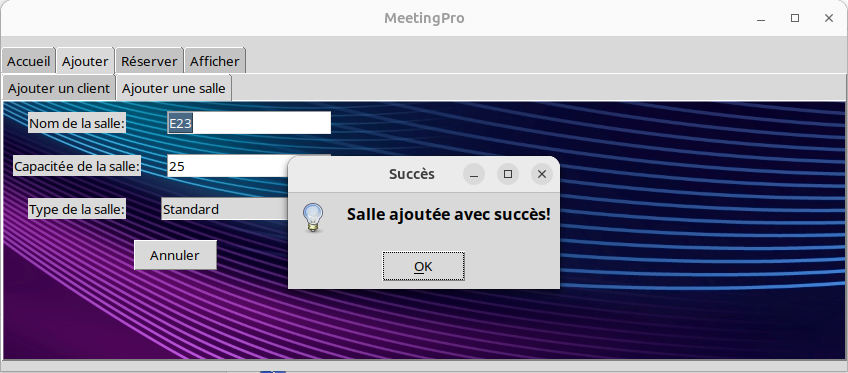
\includegraphics[width=\textwidth]{screenshot3.jpg}
        \caption{Information de réussite d'ajout de salle}
    \end{subfigure}
    \caption{Captures d'écran de l'application MeetingPro}
\end{figure}

\section{Difficultés rencontrées}

Le projet a soulevé plusieurs défis :
\begin{itemize}
    \item \textbf{Apprentissage de Tkinter et JSON} : la documentation étant parfois limitée, la courbe d’apprentissage a été marquée, notamment pour lier efficacement l’interface aux données.
    \item \textbf{Interface dynamique} : adapter les widgets Tkinter à des modifications en temps réel fut complexe.
    \item \textbf{Changement d’UI en cours de projet} : une nouvelle directive imposée par nos enseignants nous a contraints à revoir intégralement l’approche de l’interface, entraînant un travail de refonte important.
    \item \textbf{Adaptation du contrôleur} : l'interfaçage avec l’UI a nécessité des ajustements non anticipés malgré une modélisation initiale rigoureuse.
\end{itemize}

\section{Perspectives}

Nous avions prévu d'ajouter un \textbf{script de compilation} pour générer des exécutables utilisables sous Linux et Windows. Faute de temps, cette fonctionnalité n’a pas pu être intégrée, mais pourrait constituer une évolution future du projet.

\newpage
\section*{Références}
\nocite{*}
\printbibliography

\end{document}
